\documentclass[12pt]{article}

\usepackage[utf8]{inputenc}
\usepackage[T2A]{fontenc}
\usepackage[english,russian]{babel}
\usepackage{amssymb}
\usepackage{graphicx}
\graphicspath{ {images/} }

\textwidth=431pt
\textheight=600pt
\hoffset=-30pt
\voffset=-30pt

\usepackage{graphicx}
\usepackage{amsmath}
\makeatletter
\renewcommand{\@oddhead}{%
\vbox{%
\hbox to \textwidth{\strut \textit{Decision Making, Problem set 2, Usvyatsov Mikhail} \hfill }
%\hbox to\textwidth{Лист\hfill Страница~\arabic{page}~из 2}
\hrule
\vspace{12pt}
}}
\renewcommand{\@oddfoot}{}
\makeatother


\begin{document}

%\tableofcontents

%\newpage

\begin{center}
\textbf{Problem Set 2;\\
due Monday September 14}
\end{center}

\bigskip
	
\textbf{Exercise 1}		
Let $X$ have a normal distribution with mean $\mu$ and variance $\sigma^2$. Find the 
probability density function of $Y = e^X$ (This is known as a lognormal distribution). 
Confirm your answer for $\mu = 0$ and $\sigma^2 = 1$ by simulations.
\medskip
		
\textbf{Solution}

$f_Y\left(y\right)=\dfrac{dg^{-1}\left(y\right)}{dy}f_X\left(g^{-1}\left(y\right)\right)$

$g\left(x\right)=e^{-x}$, $g^{-1}\left(y\right)=ln\left(y\right)$\\

Hence,

$f_{y}=\dfrac{1}{\sqrt{2\pi}}e^{-\dfrac{\left(ln\left(y\right)-\mu\right)^2}{2\sigma^2}}$

\bigskip

\textbf{Exercise 2}
Suppose the random variable $X_n$ is equal to the total obtained in the $n$ tosses of a symmetric die.
\newcounter{acounter}
\begin{list}{(\alph{acounter})~}{\usecounter{acounter}}
\item Applying Chebyshev's inequality, estimate $P\left(\left|X_n - 3.5\right| > \epsilon\right)$. For what values of n one has $P\left(\left|X_n - 3.5\right| > \epsilon\right)\leq0.1$?
\item Applying the central limit theorem, choose n such that the inequality $P\left(\left|X_n - 3.5\right| > 0.1\right)\leq 0.1$ in $2a$ holds.
\end{list}

\medskip		

\textbf{Solution}

\newcounter{bcounter}
\begin{list}{(\alph{bcounter})~}{\usecounter{bcounter}}
\item 

$\sigma_{X}^2=E\left(X^2\right)-\left(E\left(X\right)\right)^2 = \dfrac{1}{6}\left(1 + 4 + 9 + 16 + 25 + 36\right)-\dfrac{1}{6}\left(1+2+3+4+5+6\right) = \dfrac{91}{6}-3.5^2 = \dfrac{35}{12}$,

$Var\left(\dfrac{X_n}{n}\right)=\dfrac{\sigma_{X}^2}{n} = \dfrac{35}{12n}$,

According to the Chebyshev's inequality:

$P\left(\left|\dfrac{X_n}{n}-3.5\right|>\epsilon\right)\leq\dfrac{35}{12n\epsilon^2}$

\item

$P\left(\left|\dfrac{X_n}{n}-3.5\right|> 0.1\right)=P\left(\dfrac{\sqrt{n}}{\sigma}\left|\dfrac{X_n}{n}-3.5\right|> \dfrac{0.1\sqrt{n}}{\sigma}\right)\approx P\left(\left|N\left(0,1\right)\right|>\dfrac{0.1\sqrt{n}}{\sigma}\right)$

$P\left(\left|N\left(0,1\right)\right|>\dfrac{0.1\sqrt{n}}{\sigma}\right) = 2\left(1-\Phi\left(\dfrac{0.1\sqrt{n}}{\sigma}\right)\right) = 2\left(1-\Phi\left(\dfrac{0.1\sqrt{n}}{1.71}\right)\right) = 2\left(1-\Phi\left(0.058\sqrt{n}\right)\right) $

\end{list}

\bigskip

\textbf{Exercise 3}

Suppose that $X_i ~ i.i.d\ N\left(0, 1\right)$ and let $s_n^2 = \dfrac{\sum_{i = 1}^n X_i^2}{n}$.

\newcounter{ccounter}
\begin{list}{(\alph{ccounter})~}{\usecounter{ccounter}}
\item 
Show that $s_n^2 \xrightarrow{p} 1$.

\item Show that $\sqrt{n}\left(s_n^2 - 1\right) \Rightarrow N \left(0, \omega^2 \right)$, and derive an expression for $\omega^2$.

\item Suppose $n = 15$, find $P\left(s_n^2 \leq 0.73\right)$ using an exact calculation.
\item Redo part (c) using the normal approximation that you developed in (b).
\item Let $A_n^2 = \dfrac{\sum_{i = 1}^n\left(X_i-\overline{X_n}\right)^2}{n-1}$
Show that $A_n^2 \rightarrow 1$.
\end{list}
The next problem illustrates the how the difference in the rate at which the tail of the probability density function goes to zero affects the rate of convergence in central limit theorems.
\medskip		

\textbf{Solution}
\newcounter{dcounter}
\begin{list}{(\alph{dcounter})~}{\usecounter{dcounter}}
\item $s_n^2 = \dfrac{\sum_{i = 1}^n X_i^2}{n}=\dfrac{\sum_{i = 1}^n\left(X_i^2\right)}{n}$

According to $N\left(0, 1\right)$ the $E\left(X_i\right)=0$. Hence, 

$s_n^2=E\left(X_i^2\right)-\left(E\left(X_i\right)\right)^2 = Var\left(X_i\right) = 1$

\item $Var\left(X_i^2\right) = E\left(X_i^4\right)-\left(E\left(X_i^2\right)\right)^2=\sigma^4\left(p-1\right)!!-1=3-1=2$

$\dfrac{\sqrt{n}\left(s_n^2-1\right)}{\sqrt{Var\left(X_i^2\right)}}=\dfrac{\sqrt{n}\left(s_n^2 - 1\right)}{\sqrt{Var\left(X_i^2\right)}} = \sqrt{\dfrac{n}{Var\left(X_i^2\right)}}\left(s_n^2-1\right) = \sqrt{\dfrac{n}{Var\left(X_i^2\right)}} \left(\dfrac{\sum_{i = 1}^n X_i^2}{n} - \left(E\left(X_i\right)\right)^2\right)$

$Var\left(X_i^2\right) = \omega^2$

$\sqrt{\dfrac{n}{\omega^2}} \left(\dfrac{\sum_{i = 1}^n X_i^2}{n} - \left(E\left(X_i\right)\right)^2\right)\rightarrow N\left(0,1\right)$

$\sqrt{n} \left(\dfrac{\sum_{i = 1}^n X_i^2}{n} - \left(E\left(X_i\right)\right)^2\right)\rightarrow \omega N\left(0,1\right)$

$\sqrt{n} \left(\dfrac{\sum_{i = 1}^n X_i^2}{n} - \left(E\left(X_i\right)\right)^2\right)\rightarrow  N\left(0,\omega^2\right)$, where $\omega^2=2$


\item $\sum_{i = 1}^{n}X_i^2$ - it's $\chi^2$ distribution with n dimension of freedom. Hence, 

$P\left(s_n^2\leq 0.73\right)\approx P\left(\dfrac{\chi^2}{n}\leq 0.73\right)=P\left(\chi^2\leq 0.73n\right)$

For n = 15

$P\left(\chi^2\leq 10.95\right)=\dfrac{\gamma\left(\dfrac{15}{2}, \dfrac{10.95}{2}\right)}{\Gamma\left(\dfrac{15}{2}\right)}=0.756$

\item $P\left(s_n^2\leq 0.73\right) = P\left(s_n^2-1\leq 0.73-1\right) = P\left(\dfrac{\sqrt{n}\left(s_n^2-1\right)}{\omega}\leq \dfrac{\sqrt{n}\left(0.73-1\right)}{\omega}\right)$

$P\left(\dfrac{\sqrt{n}\left(s_n^2-1\right)}{\omega}\leq \dfrac{\sqrt{n}\left(0.73-1\right)}{\omega}\right)\approx P\left(N\left(0, 1\right)\leq -\dfrac{\sqrt{15}\cdot 0.27}{\sqrt{2}}\right)$

$P\left(N\left(0, 1\right)\leq -\dfrac{\sqrt{15}\cdot 0.27}{\sqrt{2}}\right)=P\left(N\left(0, 1\right)\geq \dfrac{\sqrt{15}\cdot 0.27}{\sqrt{2}}\right) = 1 - P\left(N\left(0, 1\right)\leq \dfrac{\sqrt{15}\cdot 0.27}{\sqrt{2}}\right) = 1-\Phi\left(\dfrac{\sqrt{15}\cdot 0.27}{\sqrt{2}}\right)=1-\Phi\left(0.74\right) = 1-0.27 = 0.73$

\item $A_n^2 = \dfrac{\sum_{i = 1}^n\left(X_i-\overline{X_n}\right)^2}{n-1} = var(\hat{X})$

$\lim_{x \to \infty} var(\hat{X}) = var(X) = 1$

So $A_n^2 = 1$,  QED
\end{list}

\bigskip

\textbf{Exercise 4}

Let $X_1, X_2,\cdots$ be a sequence of independent uniform random variables, and define $Y_n=\sqrt{\dfrac{12}{n}}\sum_{i=1}^n\left(X_i-\dfrac{1}{2}\right)$, and let $Z_1, Z_2,\cdots$ be a sequence exponential random variables, and define $W_n = \dfrac{\sum_{i=1}^n\left(Z_i-1\right)}{\sqrt{n}}$

\newcounter{icounter}
\begin{list}{(\alph{icounter})~}{\usecounter{icounter}}
\item Calculate the mean and variance and third moment of $Y_n$ and $W_n$.
\item Calculate for $n=1$ the probability that $Y_n$ and $W_n$ are larger
than $1.96$ and the probability they are smaller than $-1.96$.
\item Estimate the probability that $Y_n$ and $W_n$ are larger than 1.96 and the probability they are smaller than $-1.96$ by drawing $10000$ random variables from their respective distributions (for $n = 1$).
\item Repeat the previous exercise for $n=2$, $n=5$ and $n=100$. Which of the two sequences converges to a normal distribution faster?
\end{list}
\medskip

\textbf{Solution}
\newcounter{fcounter}
\begin{list}{(\alph{fcounter})~}{\usecounter{fcounter}}
\item Lets find $E\left(X_i\right)$ and $E\left(X_i^2\right)$

$E\left(X_i\right)=\int_{-\infty}^{\infty}xf\left(x\right)dx=\int_{a}^{b}xdx=\dfrac{x^2}{2}\vert_a^b=\dfrac{b^2}{2}-\dfrac{a^2}{2}$

For $x \in \left[0, 1\right]$ $E\left(X_i\right)=\dfrac{1}{2}$

$E\left(X_i^2\right)=\int_{-\infty}^{\infty}x^2f\left(x\right)dx = \int_{a}^{b}x^2dx = \dfrac{x^3}{3}\vert_a^b=\dfrac{b^3}{3}-\dfrac{a^3}{3}$

For $x \in \left[0, 1\right]$ $E\left(X_i^2\right)=\dfrac{1}{3}$

\medskip

Lets find expectation of $Y_n$:

$E\left(Y_n\right)=E\left(\dfrac{12}{n}\sum_{i = 1}^n\left(X_i-\dfrac{1}{2}\right)\right)=\dfrac{12}{n}E\left(\sum_{i=1}^n\left(X_i-\dfrac{1}{2}\right)\right)=\dfrac{12}{n}\sum_{i=1}^nE\left(X_i-\dfrac{1}{2}\right)=\sqrt{\dfrac{12}{n}}\sum_{i = 1}^n\left(E\left(X_i\right)-E\left(\dfrac{1}{2}\right)\right)=\sqrt{\dfrac{12}{n}}\sum_{i = 1}^n\left(\dfrac{1}{2}-\dfrac{1}{2}\right) = 0$

\medskip

Lets find variance of $Y_n$:

$Var(X_i) = E\left(X_i^2\right) - \left(E\left(X_i\right)\right)^2 = \dfrac{1}{3}-\dfrac{1}{4} = \dfrac{1}{12}$

$Var\left(Y_n\right) = Var\left(\sqrt{\dfrac{12}{n}}\sum_{i=1}^n\left(X_i-\dfrac{1}{2}\right)\right)=\dfrac{12}{n}Var\left(\sum_{i=1}^n\left(X_i-\dfrac{1}{2}\right)\right)=\dfrac{12}{n}\sum_{i=1}^n Var\left(X_i\right) = \dfrac{12}{n}\cdot n\cdot Var\left(X_i\right) = \dfrac{12}{n}\cdot \dfrac{1}{12}\cdot n = 1$

\medskip

Lets find third moment of $Y_n$:

$E\left(Y_n^3\right)=E\left(\left(\sqrt{\dfrac{12}{n}}\sum_{i=1}^n\left(X_i-\dfrac{1}{2}\right)\right)^3\right)=\left(\dfrac{12}{n}\right)^{1.5}E\left(\left(\sum_{i=1}^n\left(X_i-\dfrac{1}{2}\right)\right)^3\right)=\left(\dfrac{12}{n}\right)^{1.5} \sum_{i = 1}^n\sum_{j = 1}^n\sum_{k = 1}^n E\left(X_i-\dfrac{1}{2}\right)\left(X_j-\dfrac{1}{2}\right)\left(X_k-\dfrac{1}{2}\right)=\left(\dfrac{12}{n}\right)^{1.5}\left(E\left(X_i-\dfrac{1}{2}\right)\right)^3=\left(\dfrac{12}{n}\right)^{1.5}\left(E\left(X_i\right)-E\left(\dfrac{1}{2}\right)\right) = \left(\dfrac{12}{n}\right)^{1.5} \cdot 0 = 0$

\medskip

Lets calculate expectation and variance of $Z_i$

$E\left(Z_i\right)=\int_0^{\infty}x\cdot e^{-x}dx = e^{-x}\left(-x-1\right)\vert_0^{\infty}=1$

$E\left(Z_i^2\right)=\int_0^{\infty}x^2\cdot e^{-x}dx = 2$

$Var\left(Z_i\right)=E\left(X_i^2\right)-\left(E\left(Z_i\right)\right)^2=2-1=1$

\medskip

Lets find expectation of $W_n$:

$E\left(W_n\right)=E\left(\dfrac{\sum_{i=1}^n\left(Z_i-1\right)}{\sqrt{n}}\right)=\dfrac{1}{\sqrt{n}}\sum_{i=1}^n\left(E\left(Z_i\right)-E\left(1\right)\right) = \dfrac{n}{\sqrt{n}}\cdot \left(1-1\right)=0$

\medskip

Lets find variance of $W_n$:

$Var\left(W_n\right)=Var\left(\dfrac{1}{\sqrt{n}}\sum_{i=1}^n\left(Z_i-1\right)\right)=\dfrac{1}{n}Var\left(\sum_{i=1}^n\left(Z_i-1\right)\right)=\dfrac{1}{n}\sum_{i=1}^n Var\left(Z_i\right)=\dfrac{1}{n}\cdot n \cdot 1 = 1$

\medskip 

Lets find third moment of $W_n$:

$E\left(W_n^3\right)=E\left(\left(\dfrac{Z_i-1}{\sqrt{n}}\right)^3\right)=\left(\dfrac{1}{\sqrt{n}}\right)^3 E\left(\left(Z_i-1\right)^3\right)=\left(\dfrac{1}{\sqrt{n}}\right)^3 \left(E\left(Z_i-1\right)\right)^3=\left(\dfrac{1}{\sqrt{n}}\right)^3\left(E\left(Z_i\right)-E\left(1\right)\right)^3=\left(\dfrac{1}{\sqrt{n}}\right)^3\left(1-1\right)=0$

\item 
\newcounter{gcounter}
\begin{list}{\arabic{gcounter})~}{\usecounter{gcounter}}
\item $P\left(\sqrt{12}\left(X_i-\dfrac{1}{2}\right)\leq -1.96\right)=P\left(X_i \leq \dfrac{-1.96}{\sqrt{12}}+\dfrac{1}{2}\right)=P\left(X_i\leq 0.0658\right)$

$P\left(X_i\leq 0.0658\right) = 0$

\item $P\left(\sqrt{12}\left(X_i-\dfrac{1}{2}\right)\geq 1.96\right)=1-P\left(\sqrt{12}\left(X_i-\dfrac{1}{2}\right)\leq 1.96\right)=1-P\left(X_i \leq \dfrac{1.96}{\sqrt{12}}+\dfrac{1}{2}\right)=1-1=0$

\item $P\left(Z_i-1\leq -1.96\right)=p\left(Z_i \leq -0.96\right) = 0$

\item $P\left(Z_i-1\geq 1.96\right)=P\left(Z_i\geq 2.96\right)=1-P\left(Z_i\leq 2.96\right)=1-1+e^{-x}=0.0518$
\end{list}

\item

$Y_n = \sqrt{12}*(X-0.5)$
$W_n = Z - 1$

It was generated 10000 uniform random variables in vector X and the same sizу exponential distributed vector Z.

We can estimate the probability by processing the real data.

$P(Y_n > 1.96) = 0$

$P(W_n > 1.96) = 0.0513$

$P(Y_n < -1.96) = 0$

$P(W_n < -1.96) = 0$ 

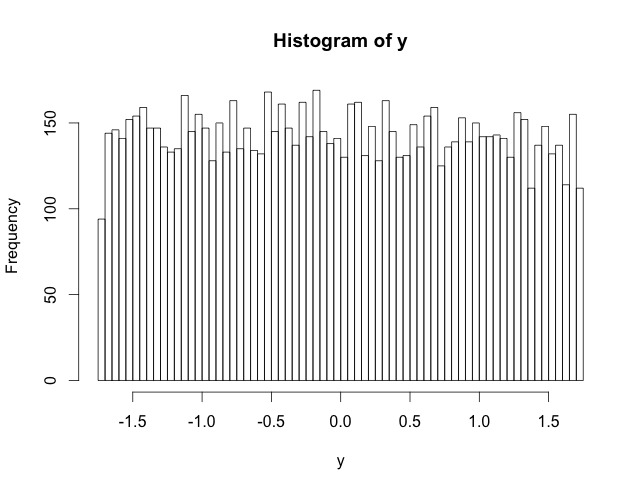
\includegraphics[width=1\textwidth]{Rplot.png}
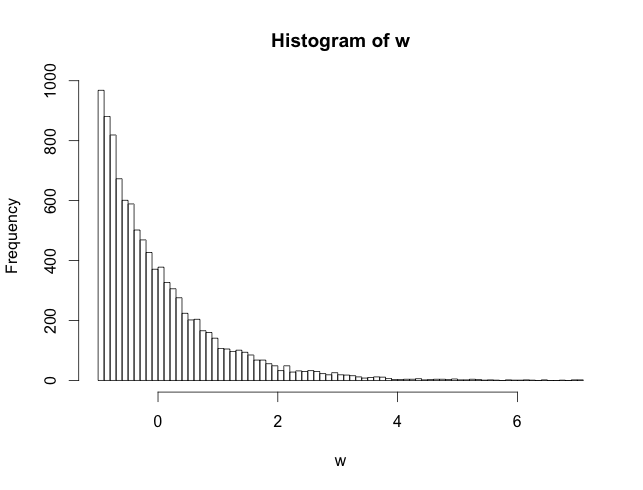
\includegraphics[width=1\textwidth]{Rplot04.png}

\item

n = 2

$P(Y_n > 1.96) = 0.0187$

$P(W_n > 1.96) = 0.0477$

$P(Y_n < -1.96) = 0.0205$

$P(W_n < -1.96) = 0$ 

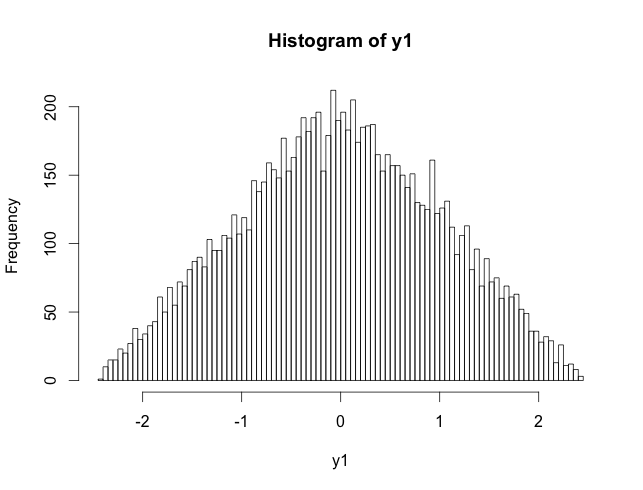
\includegraphics[width=1\textwidth]{Rplot01.png}
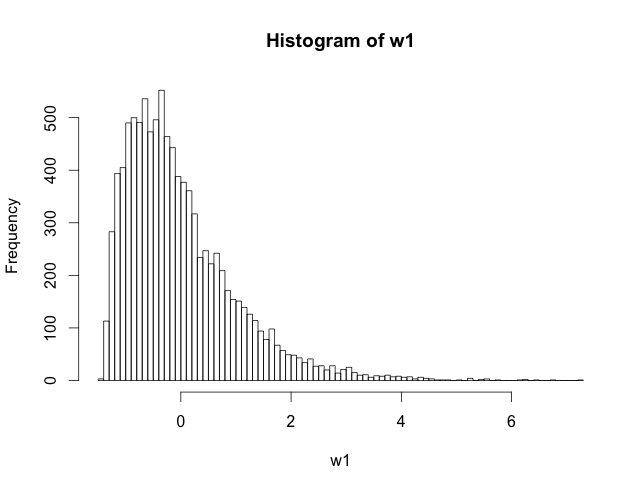
\includegraphics[width=1\textwidth]{Rplot05.png}

n = 5

$P(Y_n > 1.96) = 0.0278$

$P(W_n > 1.96) = 0.0402$

$P(Y_n < -1.96) = 0.0231$

$P(W_n < -1.96) = 4e-04$ 

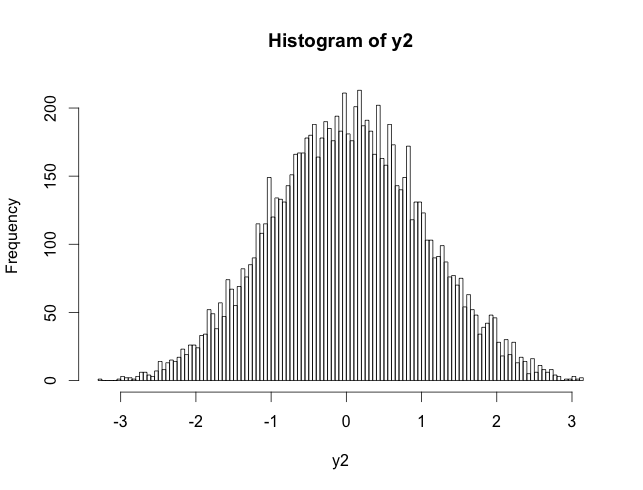
\includegraphics[width=1\textwidth]{Rplot02.png}
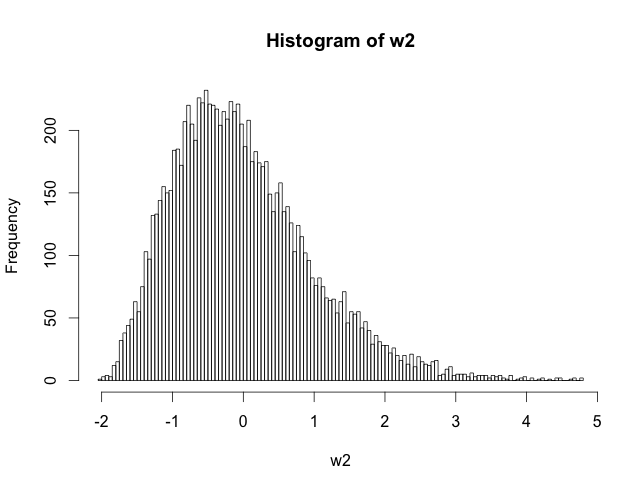
\includegraphics[width=1\textwidth]{Rplot06.png}

n = 100

$P(Y_n > 1.96) = 0.0254$

$P(W_n > 1.96) = 0.0311$

$P(Y_n < -1.96) = 0.0239$

$P(W_n < -1.96) = 0.017$ 

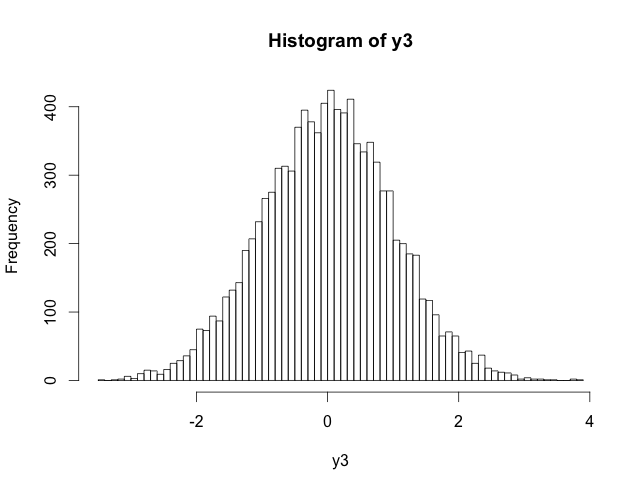
\includegraphics[width=1\textwidth]{Rplot03.png}
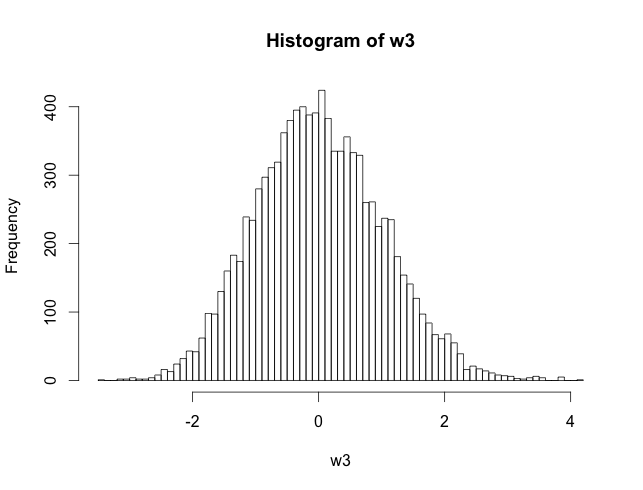
\includegraphics[width=1\textwidth]{Rplot07.png}

It is obvious that Y is closer to Normal distribution. It is well known formula to generate normal distributed values

\end{list}

\bigskip

\textbf{Exercise 5}
Suppose that $X_n \approx N\left(1, \dfrac{1}{n}\right))$ for all $n$. Use the delta method to find
an approximate normal distribution for $\sqrt{n}(e^{X_n} - e^{1})$.
\medskip

\textbf{Solution}

We have $X_n \sim N\left(1, \dfrac{1}{n}\right)$

$X_n-1 \sim N\left(0, \dfrac{1}{n}\right)$

$X_n-1 \sim \dfrac{1}{\sqrt{n}} N\left(0, 1\right)$

$\sqrt{n}\left(X_n-1\right) \sim N\left(0, 1\right)$

According to the delta-method $\sqrt{n}\left(g\left(x\right)-g\left(\theta\right)\right)~N\left(0, \sigma^2 \cdot g'\left(\theta\right)^2\right)$

Hence,

$g\left(x\right)=e^x, g'\left(x\right)=e^x$

$\sqrt{n}(e^{X_n} - e^{1})\sim N\left(0, e\right)$

\bigskip 

\textbf{Exercise 6}

In a survey of 400 likely voters, 215 responded that they would vote for the incumbent and 185 responded that they would vote for the challenger. Let p denote the fraction of all likely voters that preferred the incumbent at the time of the survey, and let $\hat{p}$ be the fraction of survey respondents that preferred the incumbent.

\newcounter{hcounter}
\begin{list}{(\alph{hcounter})~}{\usecounter{hcounter}}
\item Use the survey results to estimate $\hat{p}$.
\item Use the estimator of the variance of $\hat{p}$, $\dfrac{\hat{p}\left(1-\hat{p}\right)}{n}$, to calculate the standard error of your estimator.
\item What is the p-value for the test $H_0: p = 0.5$ vs. $H_a: p \neq 0.5$?
\item What is the p-value for the test $H_0: p = 0.5$ vs. $H_a: p > 0.5$?
\item Did the survey contain statistically significant evidence that the incumbent was ahead of the challenger at the time of the survey?
\end{list}

\medskip

\textbf{Solution}

\newcounter{jcounter}
\begin{list}{(\alph{jcounter})~}{\usecounter{jcounter}}
\item 
$\hat{p}=\dfrac{215}{400} = 0.5375$
\item
$SE(\hat{p})=\sqrt{\dfrac{\hat{p}(1 - \hat{p})}{n}} = 0.02492959$
\item
$t = \dfrac{\hat{p}-p}{SE(\hat{p})}=1.504237$

p-value = 2$\Phi(-|t|)$ = 0.132
\item
p-value = 1-$\Phi(t)$ = 0.066
\item
According to D and С we can not reject $H_0$ hypothesis because t statistic is less than 1.645. Moreover p-value is 0.066 that is bigger 0.05. So statisticaly the survey was wrong.
\end{list}
\end{document}